\documentclass[10pt]{article}
\usepackage[margin=1in]{geometry} 
\usepackage{amsmath,amsthm,amssymb,amsfonts}
\usepackage{mathtools}
\usepackage{color}
\usepackage{hyperref}
\DeclarePairedDelimiter\ceil{\lceil}{\rceil}
\renewcommand{\baselinestretch}{1.1}
\newenvironment{problem}[2][Problem]{\begin{trivlist}
\item[\hskip \labelsep {\bfseries #1}\hskip \labelsep {\bfseries #2.}]}{\end{trivlist}}

% Colors
\definecolor{blu}{rgb}{0,0,1}
\def\blu#1{{\color{blu}#1}}
\definecolor{gre}{rgb}{0,.5,0}
\def\gre#1{{\color{gre}#1}}
\definecolor{red}{rgb}{1,0,0}
\def\red#1{{\color{red}#1}}

% Math
\def\C{\mathbb{C}}
\def\E{\mathbb{E}}
\def\R{\mathbb{R}}
\def\N{\mathbb{N}}
\def\Z{\mathbb{Z}}

\def\A{\mathcal{A}}
\def\B{\mathcal{B}}
\def\D{\mathcal{D}}
\def\F{\mathcal{F}}
\def\G{\mathcal{G}}
\def\H{\mathcal{H}}
\def\L{\mathcal{L}}
\def\P{\mathcal{P}}
\def\S{\mathcal{S}}
\def\T{\mathcal{T}}
\def\a{\alpha}
\def\b{\beta}
\def\t{\tau}
\def\epsi{\epsilon}
\def\em{\emptyset}
\def\imp{\Rightarrow}
\def\limp{\Leftarrow}
\def\goes{\rightarrow}

\def\argmax{\mathop{\rm arg\,max}}
\def\argmin{\mathop{\rm arg\,min}}
\newcommand{\mat}[1]{\begin{bmatrix}#1\end{bmatrix}}
\newcommand{\alignStar}[1]{\begin{align*}#1\end{align*}}

%%
\newtheorem{thm}{Theorem}[section]
\newtheorem{cor}{Corollary}[thm]
\newtheorem{lemma}[thm]{Lemma}
\theoremstyle{definition}
\newtheorem{defn}{Definition}[section]
\newtheorem{example}{Example}[section]
\newtheorem{claim}{Claim}[section]
\newtheorem{prop}{Proposition}[section]
\newtheorem{pty}{Property}[section]
\newtheorem{remark}{Remark}[section]
\newtheorem{notation}{Notation}[section]
\newtheorem{obs}{Observation}[section]
\newcommand{\The}[2]{\begin{#1}#2\end{#1}}
\newcommand{\ord}[0]{\text{ord}}

%%
% notes
\iftrue 
\newcommand{\f}[2]{\frac{#1}{#2}}
\newcommand{\re}[1]{\frac{1}{#1}}
\newcommand{\half}[0]{\frac{1}{2}}
\newcommand{\ift}[0]{It follows that}
\newcommand{\cp}[1]{\overline{#1}}
\newcommand{\Note}[0]{\noindent\textbf{Note: }} 
\newcommand{\Claim}[0]{\noindent\textbf{Claim: }} 
\newcommand{\Lemma}[1]{\noindent\textbf{Lemma #1}: } %
\newcommand{\Ex}[0]{\noindent\textbf{Example: }} %
\newcommand{\Special}[0]{\noindent\textbf{Special case: }} %
\newcommand{\solution}[2]{\item[]\proof[Solution to #1] #2 \qedhere}
\newcommand{\legendre}[2]{\left(\frac{#1}{#2}\right)}
\newcommand{\dent}[0]{\hspace{0.5in}}
\fi

\newcommand{\sm}[0]{\setminus}
\newcommand{\set}[1]{\left\{ #1 \right\}}
\newcommand{\expect}[1]{\operatorname{E}\left[\,#1\,\right]}
\newcommand{\nl}[0]{\vspace{12pt}}
\newcommand{\rng}[2]{#1,\dots,#2}
\newcommand{\srng}[3]{#1_#2,\dots,#1_#3}
\newcommand{\st}[0]{\text{ such that }}
\newcommand{\et}[0]{\text{ and }}
\newcommand{\then}[0]{\text{ then }}
\newcommand{\forsome}[0]{\text{ for some }}
\newcommand{\floor}[1]{\lfloor #1 \rfloor}

% misc
\newcommand{\abs}[1]{\left\lvert#1\right\rvert} %
% lcm ???
\DeclareMathOperator{\lcm}{lcm} 
% blackboard bold
\newcommand{\RR}{\mathbb{R}}
\newcommand{\FF}{\mathbb{R}}
\newcommand{\QQ}{\mathbb{Q}}
\newcommand{\ZZ}{\mathbb{Z}}
\newcommand{\NN}{\mathbb{N}}
\newcommand{\CC}{\mathbb{C}}
% mathcal
\newcommand{\m}[1]{\mathcal{#1}}
% vectors
\newcommand{\vvec}[1]{\textbf{#1}} %
\newcommand{\ii}[0]{\vvec{i}} %
\newcommand{\jj}[0]{\vvec{j}} %
\newcommand{\kk}[0]{\vvec{k}} %
\newcommand{\hvec}[1]{\hat{\textbf{#1}}} %
\newcommand{\cvec}[3]{ %column vector
    \ensuremath{\left(\begin{array}{c}#1\\#2\\#3\end{array}\right)}}
\newcommand{\pfrac}[2]{\frac{\partial#1}{\partial#2}} %
\newcommand{\norm}[1]{\left\lVert#1\right\rVert} %
% dotp roduct
\makeatletter
\newcommand*\dotp{\mathpalette\dotp@{.5}}
\newcommand*\dotp@[2]{\mathbin{\vcenter{\hbox{\scalebox{#2}{$\m@th#1\bullet$}}}}}
\makeatother
% divrg and curl
\newcommand{\divrg}[0]{\nabla\dotp} %
\newcommand{\curl}[0]{\nabla\times} %

\begin{document}

\title{\vspace{-1.6cm} \huge\textbf{{Notes on Sequential Model-based Optimization}}}
\author{\large\textit{{Jingyuan Hu}}}
\date{}
\maketitle
\text{}\\
{\bf Reference}: {\it Hutter, Frank, Holger H. Hoos, and Kevin Leyton-Brown.
"Sequential model-based optimization for general algorithm configuration (extended version)."
Technical Report TR-2010–10, University of British Columbia, Computer Science, Tech. Rep. (2010).}

\tableofcontents

\section{Introduction}

\begin{itemize}
	\item Model-free algorithm configuration methods
	      \begin{itemize}
		      \item Racing: F-RACE
		      \item Iterated local search: PARAMILS
		      \item Genetic: GGA
	      \end{itemize}
	\item Model-based approaches: Sequential model-based optimization (SMBO)
	      iterates between fitting models and using them to make choices about which configurations to investigate
	\item Main Contribution: remove limitations on
	      \begin{itemize}
		      \item only supports numerical parameters
		      \item only optimizes target algorithm performance for single instances
	      \end{itemize}
	\item Two novel SMBO instantiations capable of general algorithm configuration
	      \begin{itemize}
		      \item simple model-free Random Online Adaptive Racing (ROAR)
		      \item Sequential Model-based Algorithm Configuration (SMAC)
	      \end{itemize}
\end{itemize}

\section{Random Online Aggressive Racing(ROAR)}
\label{sec:ROAR}
\begin{itemize}
	\item random: set of candidates is selected at random.
	\item online: each candidate is accepted or rejected online.
	\item aggressive: this online decision is made aggressively,
	      before enough data has been gathered to support a statistically significant conclusion.
	\item race: runs each candidate configuration only as long as necessary to
	      establish whether it is competitive.
\end{itemize}

ROAR is completely specified by the four components:
\begin{enumerate}
	\item {\it Initialize} performs a single run with the target algorithm’s default parameter configuration
	      (or a random configuration if no default is available) on an instance selected uniformly at random.
	\item {\it FitModel} procedure simply returns a constant model which is never used since ROAR is model-free.
	\item {\it SelectConfigurations} returns a single configuration sampled uniformly at random from the parameter space.
	\item {\it Intensify} \begin{itemize}
		      \item Takes as input a list of promising configurations, $\vec{\Theta}_{new}$, and compares them in turn to the current
		            incumbent configuration until a time budget for this comparison stage is reached.
		      \item  In each comparison of a new configuration, $\theta_{new}$, to the incumbent, $\theta_{inc}$, we first
		            perform an additional run for the incumbent, using a randomly selected $<$instance, seed$>$ combination.
		      \item Then, we iteratively perform runs with $\theta_{new}$ (using a doubling scheme)
		            until either $\theta_{new}$’s empirical performance is worse than that of $\theta_{inc}$ (in which case
		            we reject $\theta_{new}$) or we performed as many runs for $\theta_{new}$ as for $\theta_{inc}$ and it is still at
		            least as good as $\theta_{inc}$ (in which case we change the incumbent to $\theta_{new}$).
		      \item The $<$instance, seed$>$ combinations for $\theta_{new}$ are sampled uniformly at random from those on which
		            the incumbent has already run.
		      \item Every comparison is based on a different randomly selected subset of instances and seeds.
	      \end{itemize}
\end{enumerate}

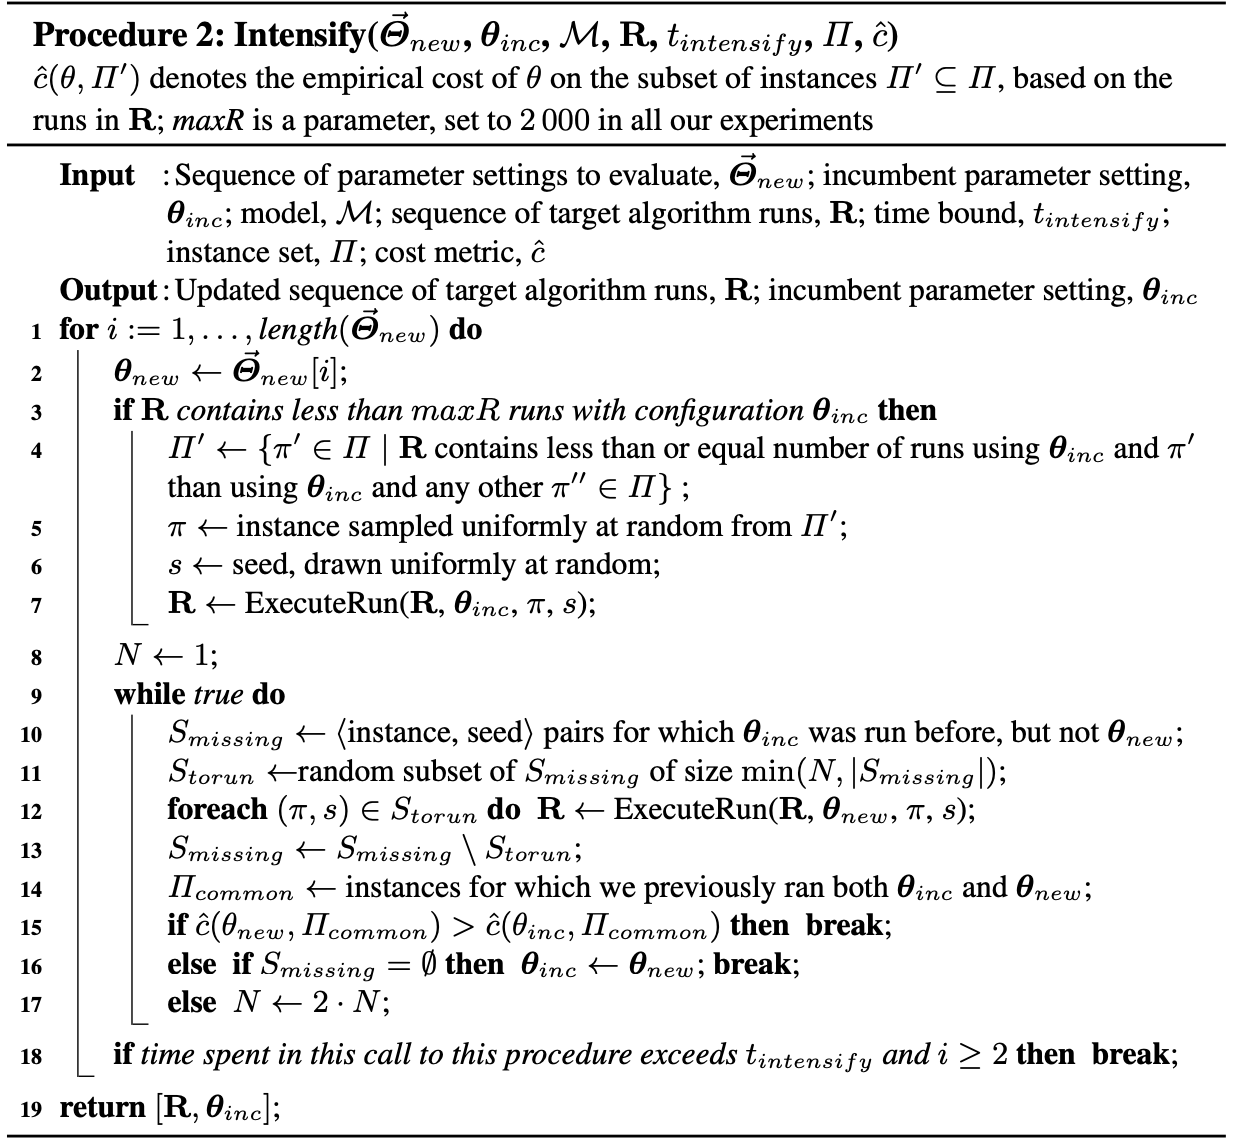
\includegraphics[width=14cm, height = 12cm]{Intensify.png}

\section{Sequential Model-based Algorithm Configuration (SMAC)}
SMAC can be understood as an extension of ROAR that selects configurations based on a model
rather than uniformly at random. It instantiates Initialize and Intensify in the same way as ROAR.\\
\text{}\\
For {\it Select Configurations}:
\begin{itemize}
	\item New model classes that supports
	      \begin{itemize}
		      \item Categorical parameters:
		            \begin{itemize}
			            \item Weighted Hamming Distance Kernel Function for GP Models
			                  \begin{equation*}
				                  K_{mixed}(\theta_i, \theta_j) =
				                  exp\big[\sum_{l \in \mathcal{P}_{cont}}(-\lambda_{l}\cdot (\theta_{i, l} - \theta_{j, l})^2)
					                  + \sum_{l \in \mathcal{P}_{cat}}(-\lambda_{l}\cdot [1- \delta(\theta_{i, l},\theta_{j, l})]) \big]
			                  \end{equation*}
			            \item Random Forests (target algorithm performance values at their leaves): construct a random forest as a set of $B$ regression
                              trees, each of which is built on $n$ data points randomly sampled with repetitions from the entire training data set. 
                              We compute the random forest’s predictive mean $\mu_{\theta}$ and variance $\sigma_{\theta}$
                              for a new configuration $\theta$ as the empirical mean and variance of its individual trees’ predictions for $\theta$.
                        \item Transformations of the Cost Metric.
		            \end{itemize}
		      \item Multiple instances: Instance Features, Predicting Performance Across Instances
	      \end{itemize}
    \item Uses the model to select a list of promising parameter configurations:
        \begin{itemize}
            \item Use model’s predictive distribution for a new configurations to compute it's $EI(\theta)$ over the incumbent
                \begin{equation*}
                    EI(\theta) := E[I_{exp}(\theta)] = f_{min} \Phi(v) - e^{\half \sigma_{\theta}^2 + \mu_{\theta}} \cdot \Phi(v - \sigma_{\theta})
                \end{equation*}
                where $v := \frac{ln(f_{min} - \mu_{\theta})}{\sigma_{\theta}}$
            \item Identify configurations with large $EI(\theta)$:
                \begin{itemize}
                    \item Previous methods: simply applied random sampling for this task  
                    (in particular, they evaluated EI for 10 000 random samples)
                    \item The author instead perform a simple {\bf multi-start local search} and consider all resulting configurations with locally maximal EI
                \end{itemize}
        \end{itemize}
    \item Detail of the multi-start local search
    \begin{itemize}
        \item Compute EI for all configuations used in previous target algorithm runs
        \item Pick the {\bf ten} configurations with maximal EI, initialize a local search at each of them
        \item To handle mixed categorical/numerical parameter spaces, they use a randomized one-exchange neighbourhood, including
        \begin{itemize}
            \item set of all configurations that differ in the value of exactly one {\bf discrete} parameter
            \item four random neighbours for each {\bf numerical} parameter: normalize the range of each numerical parameter 
            to $[0,1]$ and then sample four “neighbouring” values for numerical parameters with current value $v$ from
            a univariate Gaussian distribution with mean $v$ and standard deviation $0.2$
        \end{itemize}
        \item Evaluate EI for all neighbours at once (batch model predictions much cheaper)
        \item Stop each local search once none of the neighbours has larger EI
    \end{itemize}
    \item Also compute EI for an additional 10,000 randomly-sampled configurations, 
        and sort all 10,010 configurations in descending order of EI. (Note: For the ten initial one
        if none configuation outperforms the initial one, then it remains to be the initial one)
    \item Alternate between configurations pairs from the list (10,010) and additional configurations pairs sampled uniformly at random 
    to provide unbiased training data for future models (e.g. Random Forest) and perform intensification on it.
\end{itemize}
\Note For details of intensification, please refer to 
\hyperref[sec:ROAR]{Section 2}
\end{document}